\section{Particle Signatures in IceCube}
\label{sec:particle-signatures}
All particle signatures in IceCube can be approximated as being combinations of compact \emph{cascades} that are produced by hadronic and electromagnetic showers (see section~\ref{sec:had-showers} and \ref{sec:em-showers}), and elongated \emph{tracks} that are only produced by muons travelling through the detector.

\subsection{Neutrinos}

At energies above 10~GeV, nearly all neutrino interactions are due to Deep Inelastic Scattering (DIS) and therefore always produce at least a hadronic cascade originating at the interaction vertex.
In Neutral-Current (NC) interactions, this hadronic cascade is the only visible part of the interaction.
Charged-current (CC) interactions also produce a lepton of the same flavor of the primary neutrino.
For electron-neutrinos, this creates an electromagnetic (EM) shower that also originates at the interaction vertex.
While the direction of the EM shower and the hadronic shower might not be exactly the same, they are in practice not distinguishable by the detector and can therefore be approximated as a single cascade-like signature.
Since the directions of the particles that make up a shower are randomly distributed with a strong bias towards the direction of the primary neutrino, the angular profile of the light emission of a cascade follows a smeared Cherenkov emission profile.
At distances of several scattering lengths ($L_s\approx25\;\mathrm{m}$), this emission profile averages out and the cascade can be approximated as a single point emitting light uniformly in all directions.
The left panel of figure~\ref{fig:idealized_signatures} shows the detector response of such an idealized, perfectly symmetric cascade event.
\begin{figure}
    \centering
    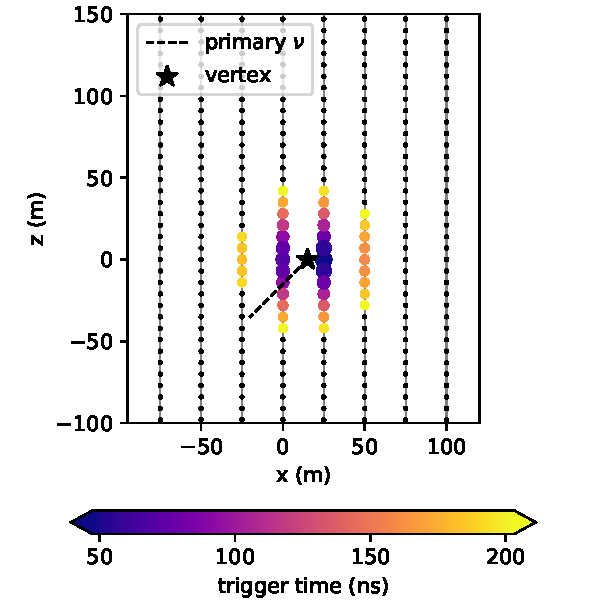
\includegraphics[width=0.49\textwidth]{figures/icecube/eventviews/idealized_cascade_view.pdf}
    \hfill
    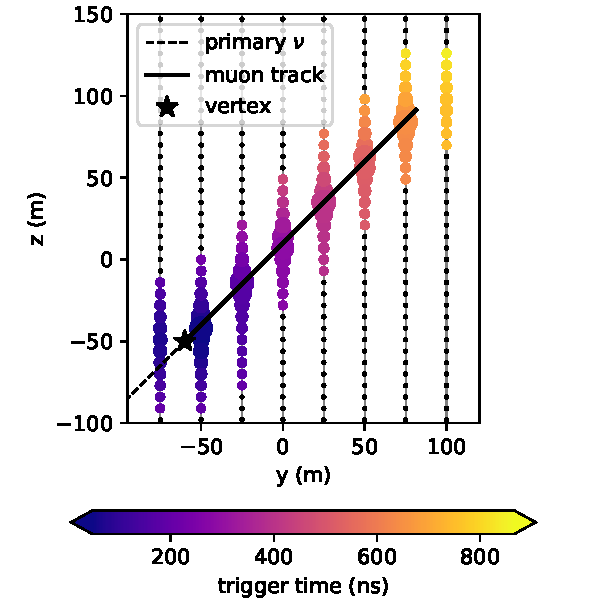
\includegraphics[width=0.49\textwidth]{figures/icecube/eventviews/idealized_track_view.pdf}
    \caption{An idealized cascade event (left) and starting track event (right) seen from the side. Each DOM that has received light is highlighted with a colored bubble, where the size is proportional the total charge seen by the DOM and the color indicates the time of the hits relative to the time at which the neutrino interaction happened.}
    \label{fig:idealized_signatures}
\end{figure}

% \begin{marginfigure}
%     \centering
%     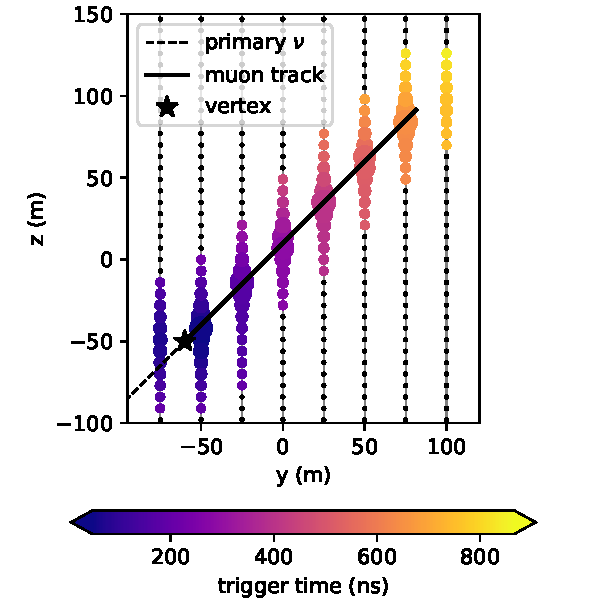
\includegraphics[width=\textwidth]{figures/icecube/eventviews/idealized_track_view.pdf}
%     \caption{An idealized \numucc-event seen from the side. Light is emitted uniformly from the interaction vertex as well as the endpoint of the track, and follows the Cherenkov cone along the track.}
%     \label{fig:idealized_track}
% \end{marginfigure}
% \begin{marginfigure}
%     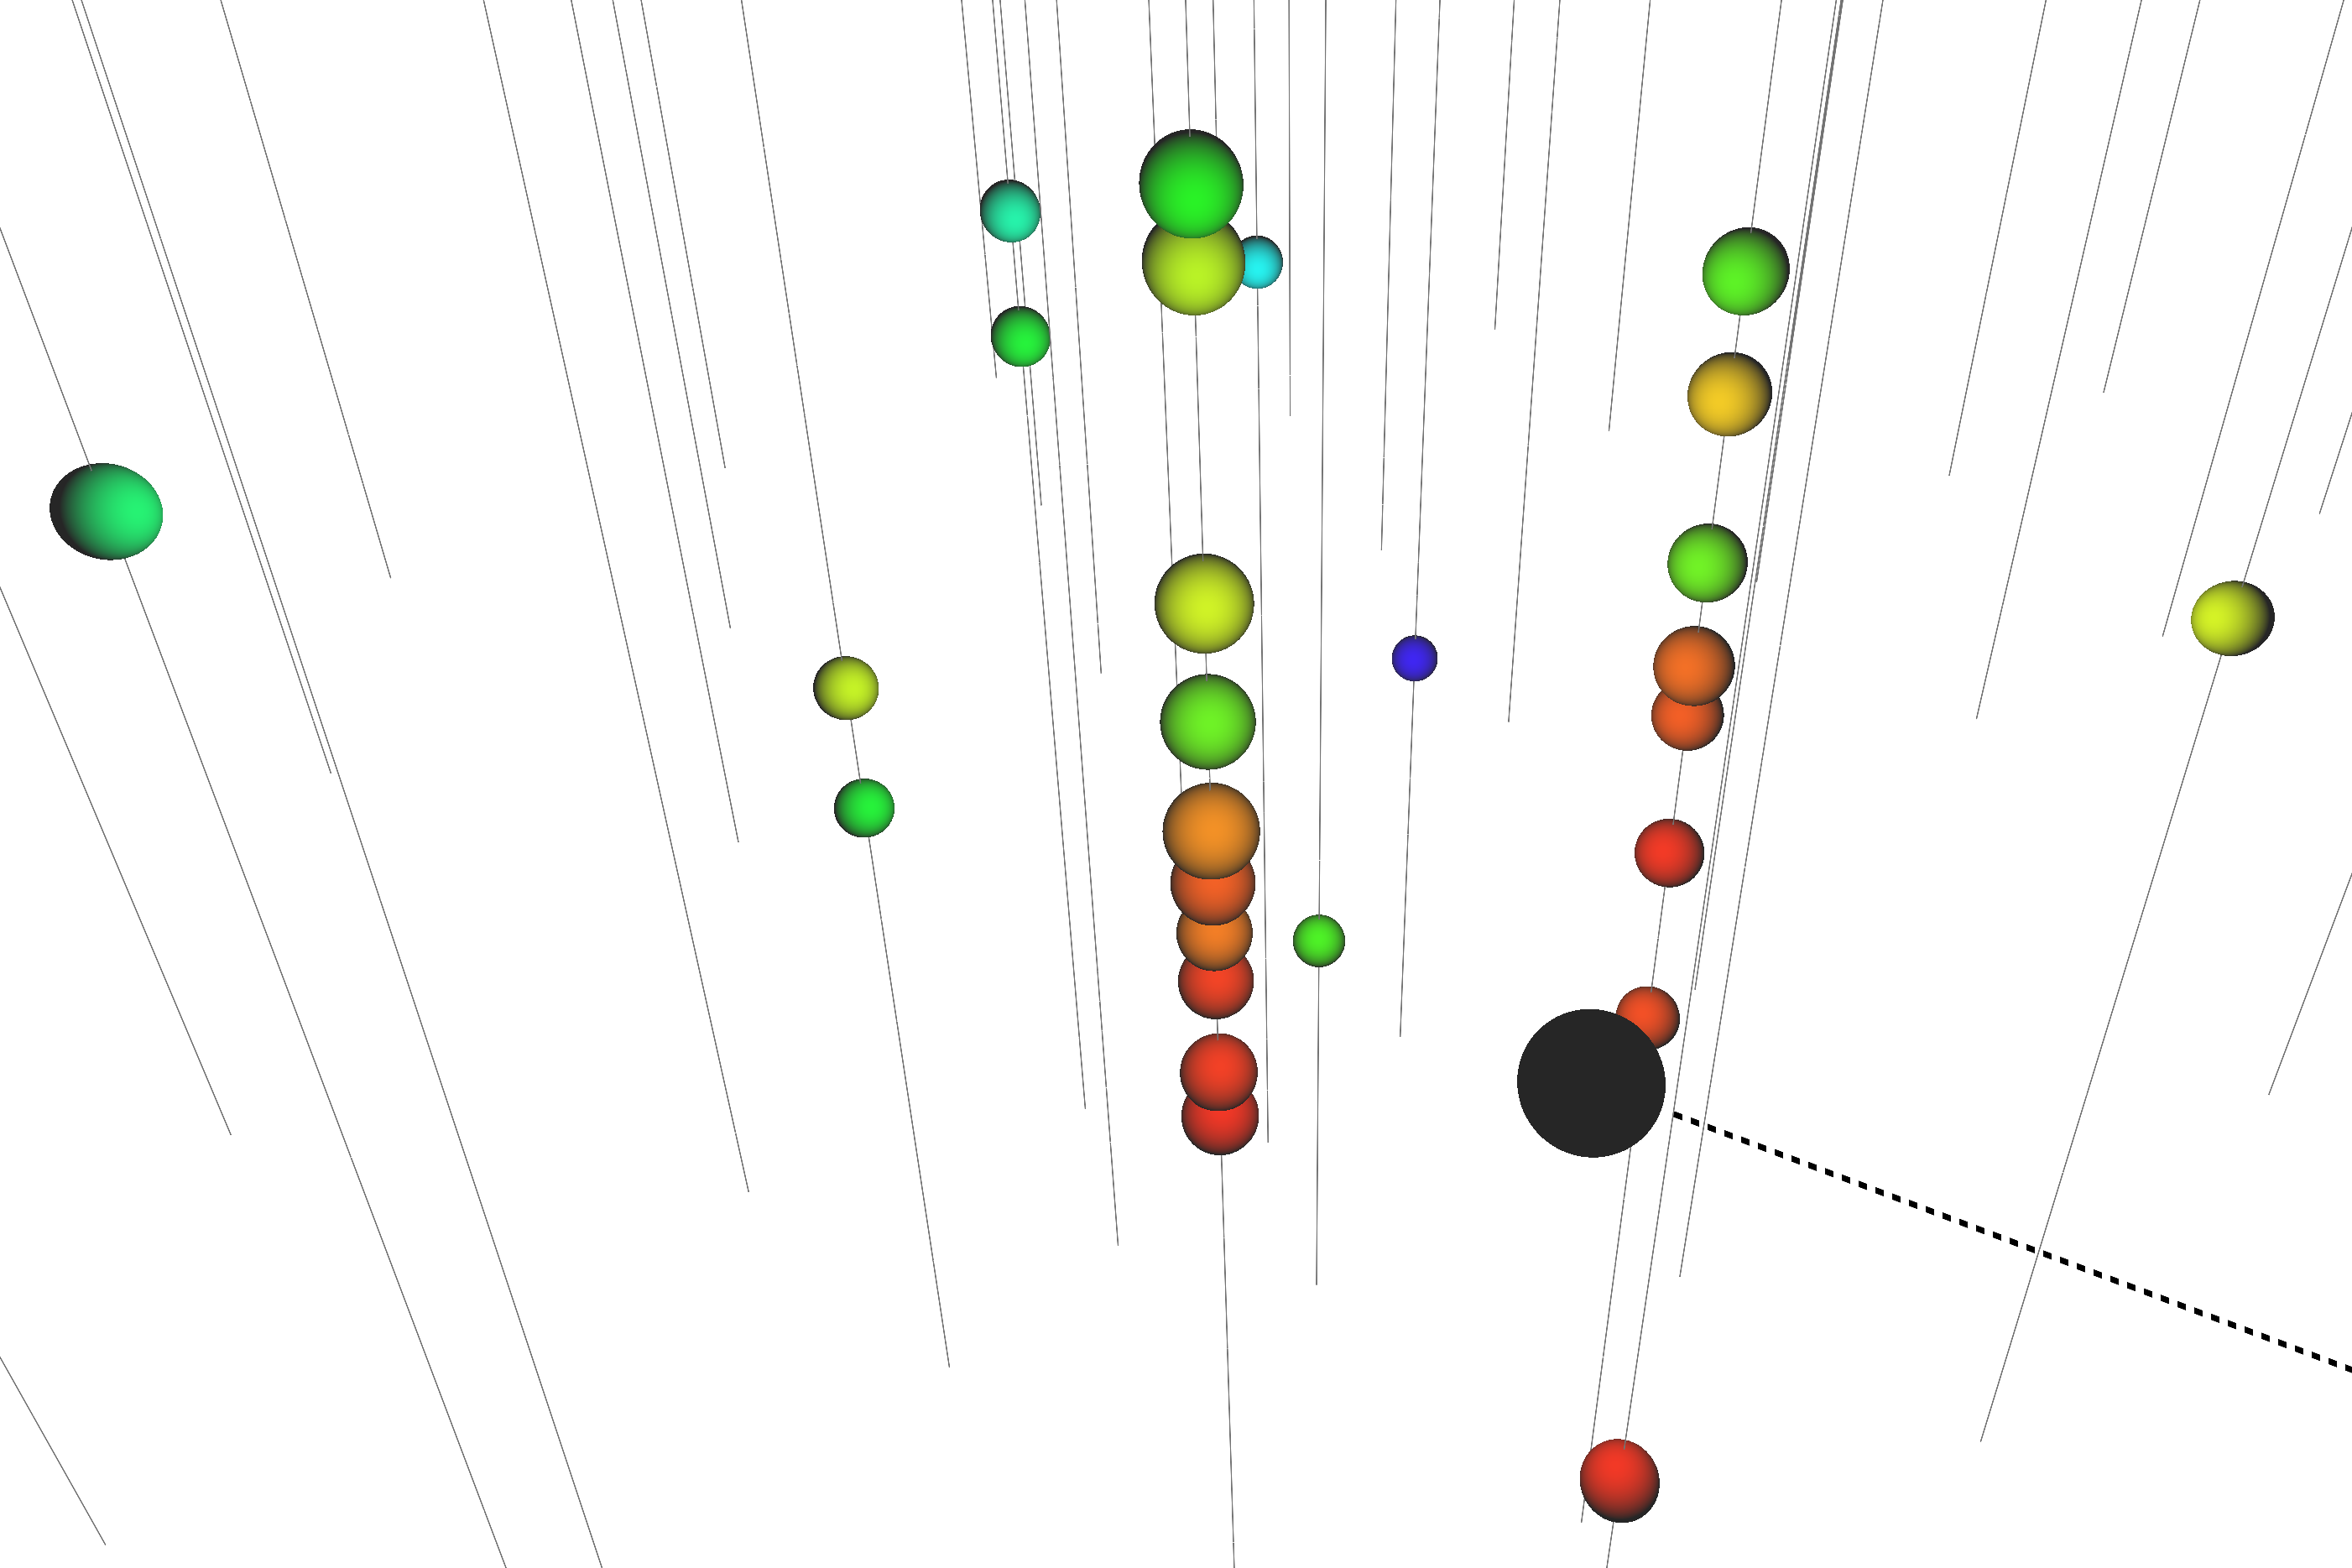
\includegraphics[width=\textwidth]{figures/icecube/eventviews/NuECC_with_neutrino_2_crop.png}
%     \caption{A simulated low energy $\nu_e$-CC neutrino interaction with an energy of 25 GeV inside the DeepCore sub-volume. The true neutrino direction is shown as the black dashed line, and the vertex as the black, round marker.}
%     \label{fig:emcasc-view}
% \end{marginfigure}
% \subsection{Tracks}
For muon-neutrinos, a muon is produced in the CC interaction which can then travel a significant distance through the ice beyond the extent of the initial hadronic shower, creating a track-like signature that sticks out of the cascade.
An idealized version of such an event is shown in the right panel of figure~\ref{fig:idealized_signatures}.

%The signal that such an interaction at an energy of 25~GeV produces in the DeepCore volume is shown in figure~\ref{fig:lowen-track-view}.
% \begin{marginfigure}
%     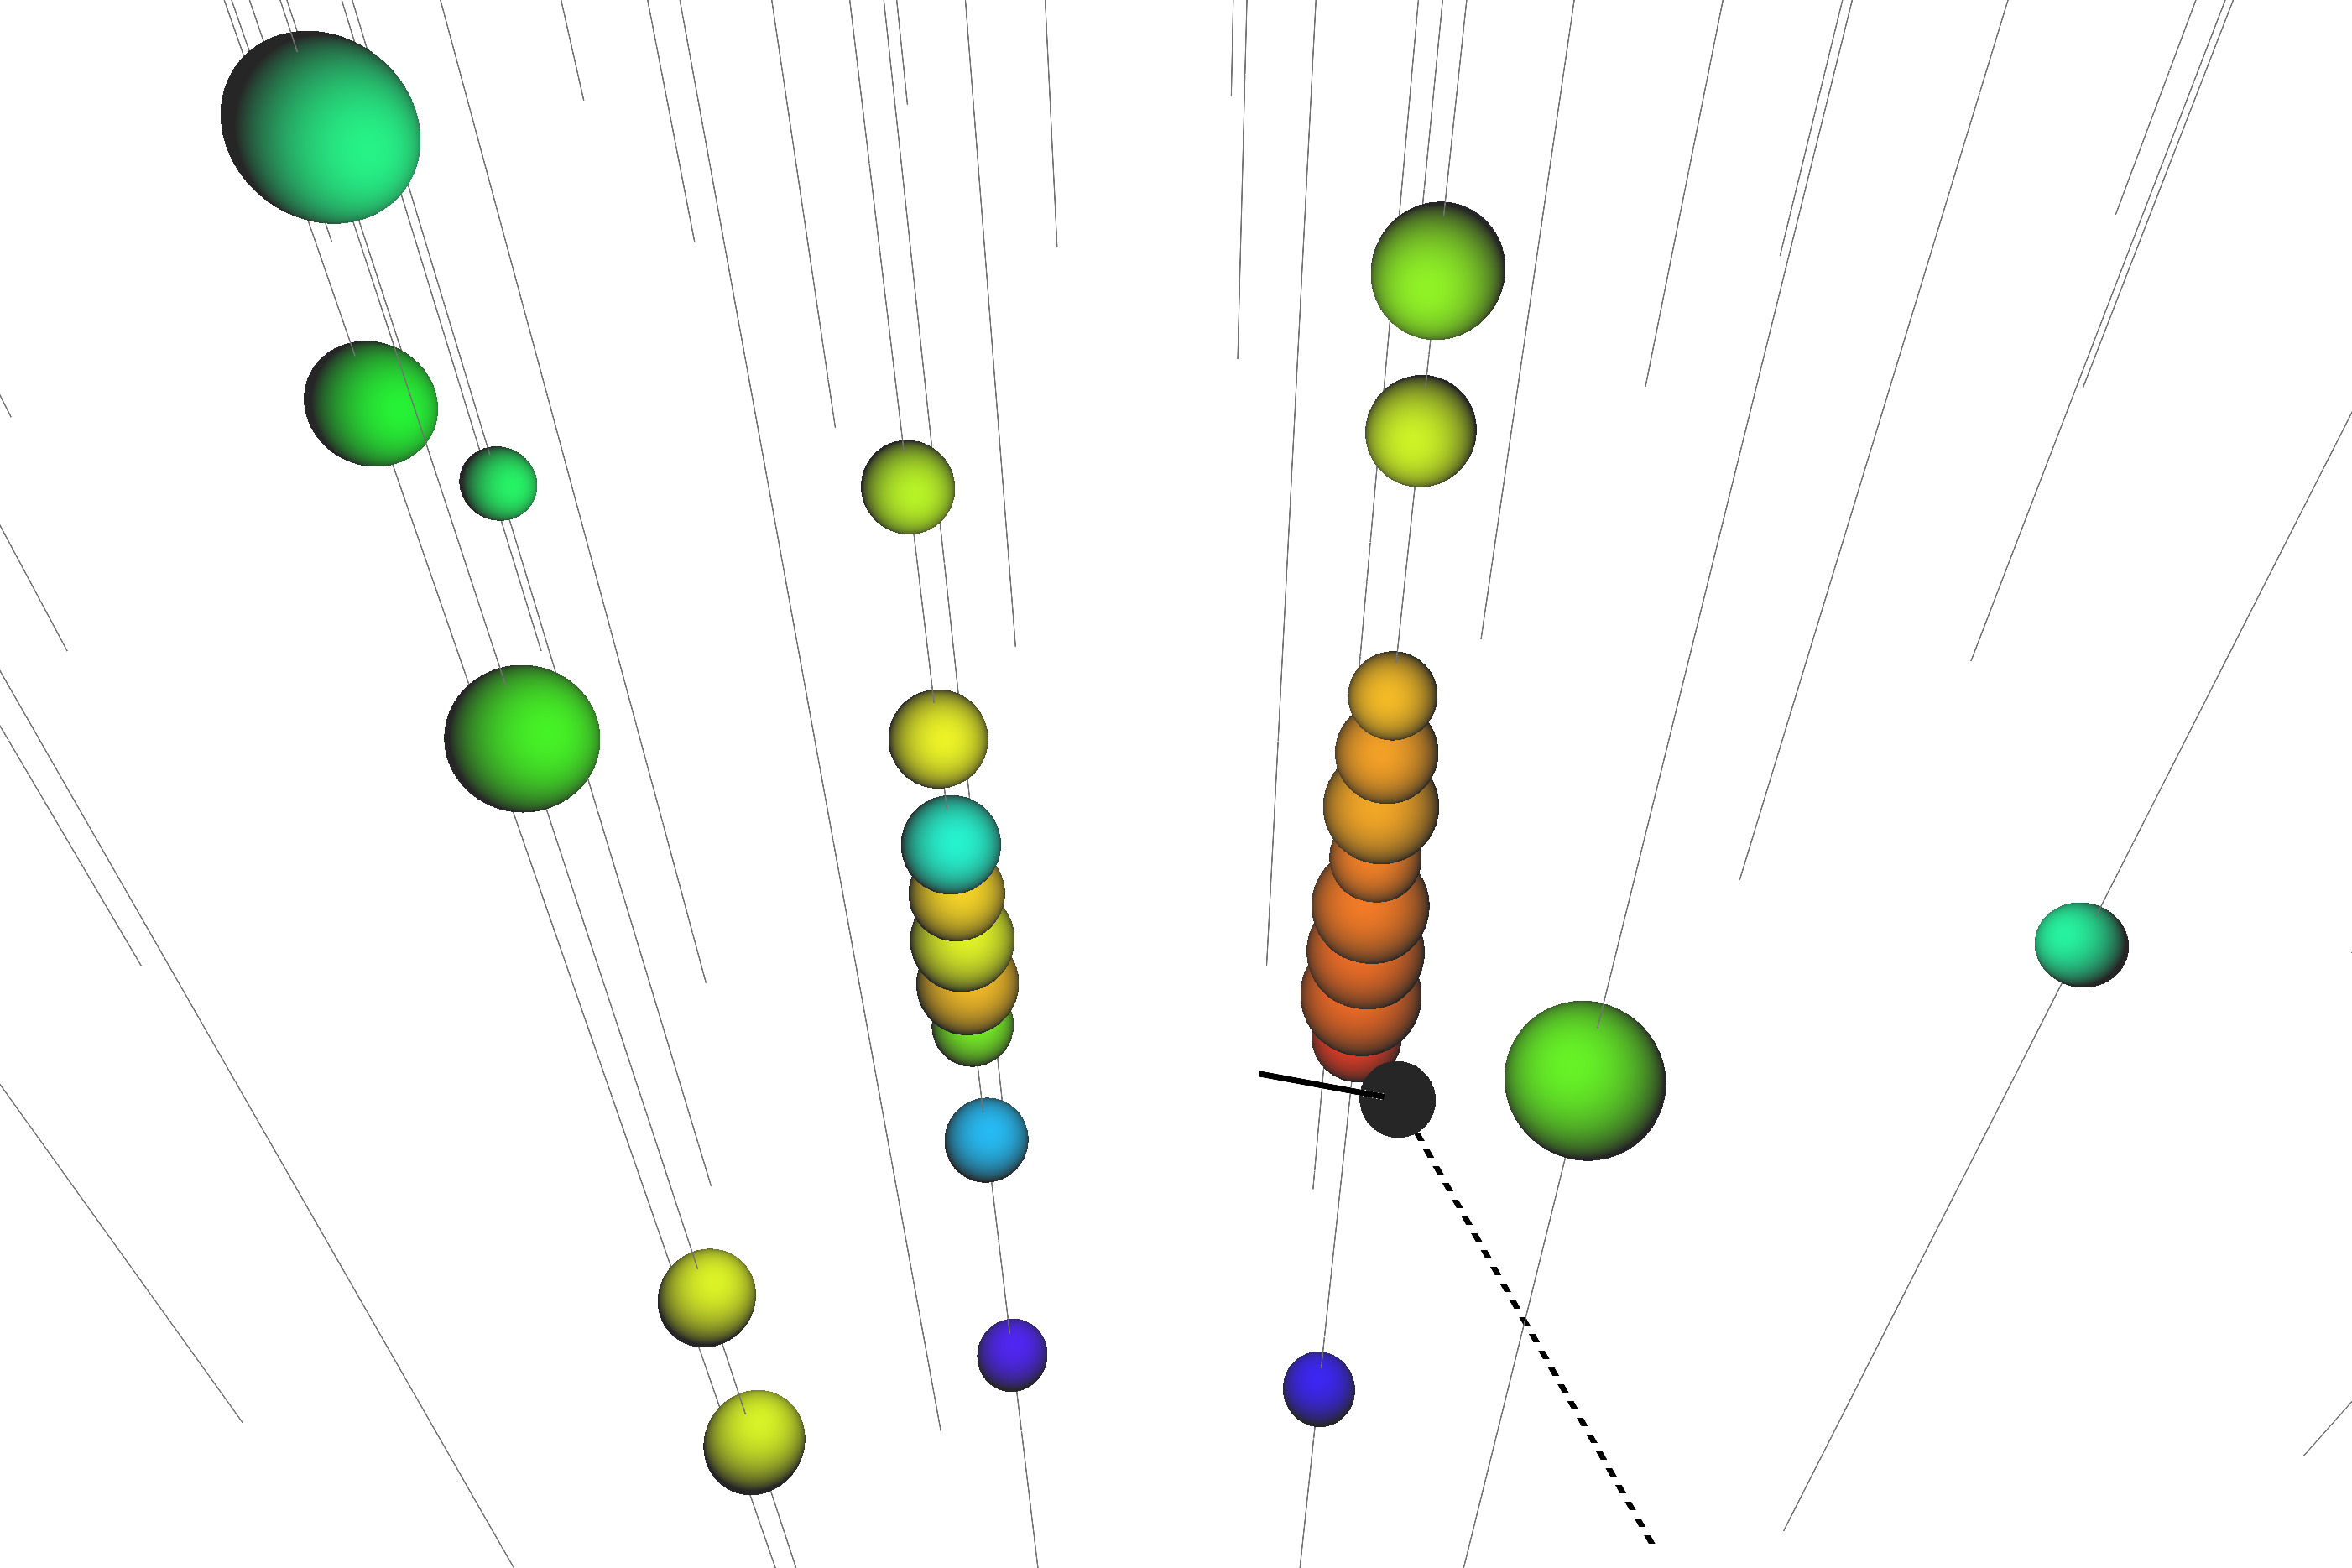
\includegraphics[width=\textwidth]{figures/icecube/eventviews/NuMuCC_with_neutrino_2_shorter_cmap_range_crop.png}
%     \caption{A simulated low energy \numucc neutrino interaction with an energy of 25~GeV inside the DeepCore sub-volume, with an outgoing 8 GeV $\mu^-$ indicated with the black, solid line (track).}
%     \label{fig:lowen-track-view}
% \end{marginfigure}
Charged-current interactions of tau-neutrinos produce a tauon that decays after a short distance, creating a second EM or hadronic shower at the point of its decay.
At TeV-scale energies, the distance covered by the tauon before its decay can be large enough to make the separation between the two showers resolvable, creating a \emph{double-bang} signature consisting of two cascades\todo{add concrete distance scale}.
At energies below 100~GeV that are more relevant to this work, however, the two cascades are too close together to be cleanly separable and they are effectively approximated as a single cascade as well.
About 17\% of tauons produce a muon upon decay, creating a track-like signature as well.
A summary of the secondary particles and corresponding signatures are given in table~\ref{tab:interaction-signatures}.
% \begin{marginfigure}
%     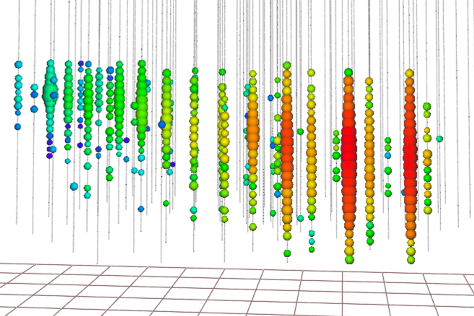
\includegraphics[width=\textwidth]{figures/icecube/eventviews/numucc_TeV_crop.png}
%     \caption{A high energy event (IceCube-170922A) with estimated energy of about 290 TeV. \cite{IceCube:2018dnn}}
%     \label{fig:txs-event}
% \end{marginfigure}

\tikzstyle{emcasc}=[shade,left color=blue!50,right color=blue!20, draw=blue]
\tikzstyle{hadcasc}=[shade,left color=red!50,right color=red!20, draw=red]
\tikzstyle{muon}=[draw=ProcessBlue, thick]
\tikzstyle{nu}=[densely dotted]
\tikzstyle{tau}=[draw=red]

\newcommand{\drawnuecc}{
    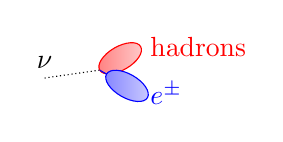
\begin{tikzpicture}
        \node (vertex) at (0, 0) {};
        \draw (-0.7, -0.1) node [anchor=south] {$\nu$} [nu] -- (vertex.center);
        \draw (vertex.center) +(0:0.3)[hadcasc,rotate=30] ellipse (0.3 and 0.15);
        \node [anchor=west,red] at (30:0.6) {hadrons};
        \draw (vertex.center) -- +(-30:0.1) +(0:0.4) [emcasc,rotate=-30] ellipse (0.3 and 0.15);
        \node [anchor=west,blue] at (-30:0.6) {$e^\pm$};
    \end{tikzpicture}
}

\newcommand{\drawnumucc}{
    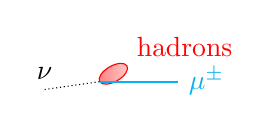
\begin{tikzpicture}
        \node (vertex) at (0, 0) {};
        \draw (-0.7, -0.1) node [anchor=south] {$\nu$} [nu] -- (vertex.center);
        \draw (vertex.center) +(0:0.2)[hadcasc,rotate=30] ellipse (0.2 and 0.1);
        \node [anchor=south west,red] at (30:0.4) {hadrons};
        \draw (vertex.center)[muon] -- +(0:1.0) node [anchor=west,ProcessBlue] {$\mu^\pm$};
    \end{tikzpicture}
}

\newcommand{\drawnutaucc}{
    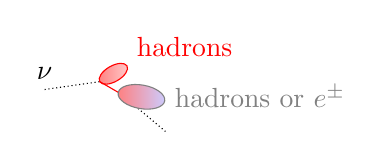
\begin{tikzpicture}
        \node (vertex) at (0, 0) {};
        \draw (-0.7, -0.1) node [anchor=south] {$\nu$} [nu] -- (vertex.center);
        \draw (vertex.center) +(0:0.2)[hadcasc,rotate=30] ellipse (0.2 and 0.1);
        \node [anchor=south west,red] at (30:0.4) {hadrons};
        \draw (vertex.center)[tau] -- +(-30:0.3) node (taudecay) {};
        \draw (taudecay.center) [nu] -- +(-40:0.75);
        \draw (taudecay.center) ++(10:0.3) [shade,left color=red!50,right color=blue!20, draw=gray,rotate=-10] ellipse (0.3 and 0.15) +(10:0.3) node [anchor=west,gray] {hadrons or $e^\pm$};
    \end{tikzpicture}
}

\newcommand{\drawnutauccmu}{
    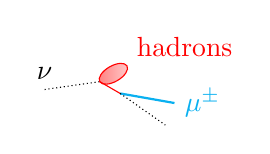
\begin{tikzpicture}
        \node (vertex) at (0, 0) {};
        \draw (-0.7, -0.1) node [anchor=south] {$\nu$} [nu] -- (vertex.center);
        \draw (vertex.center) +(0:0.2)[hadcasc,rotate=30] ellipse (0.2 and 0.1);
        \node [anchor=south west,red] at (30:0.4) {hadrons};
        \draw (vertex.center)[tau] -- +(-30:0.3);
        \draw (vertex.center) ++(-30:0.3)[muon] -- +(-10:0.7) node [anchor=west,ProcessBlue] {$\mu^\pm$};
        \draw (vertex.center) ++(-30:0.3)[nu] -- +(-35:0.7);
    \end{tikzpicture}
}

\newcommand{\drawnunc}{
    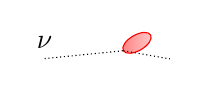
\begin{tikzpicture}
        \node (vertex) at (0, 0) {};
        \draw (-1, -0.1) node [anchor=south] {$\nu$}[nu] -- (vertex.center);
        \draw (vertex.center) +(0:0.2)[hadcasc,rotate=30] ellipse (0.2 and 0.1);
        \draw (vertex.center)[nu] -- +(-10:0.6);
    \end{tikzpicture}
}

\begin{table}
    \centering
    \begin{tabular}{p{0.1 \linewidth}cc}
         interaction & secondary particles & signature \\
         \toprule
         $\nu_e$ CC &  \drawnuecc &  cascade\\
         \midrule
         $\nu_\mu$ CC &  \drawnumucc &  cascade + track\\
         \midrule
         $\nu_\tau$ CC (83\%~BR) &  \drawnutaucc &  cascade\\
         $\nu_\tau$ CC (17\%~BR) &  \drawnutauccmu &  cascade + track\\
         \midrule
         $\nu$ NC &  \drawnunc &  cascade\\
    \end{tabular}
    \caption{Secondary particles and signatures produced by each type of neutrino interaction.}
    \label{tab:interaction-signatures}
\end{table}

\subsection{Atmospheric muons}

Atmospheric muons at energies below 100~GeV, where the dominant process of energy loss is ionization, create a single long track-like signature that can pass through the entire volume of the IceCube sensor array.
At energies above 100~GeV, radiative energy losses become more relevant that create a series of stochastically distributed cascades along the muon's trajectory.
The fraction of total energy loss that is concentrated in these cascades is referred to as \emph{stochasticity}.
Atmospheric muons also often arrive in bundles originating from a single interaction of cosmic rays with the upper atmosphere.
Within such a bundle, stochastic energy losses of individual muons may average out over its trajectory, such that the bundle as a whole can be approximated as a single long track with a relatively low stochasticity.
